\chapter{Background}
\label{chap:background}

XXX We need to decide, y'know, what goes into the background section.

What did we say in the outline?

\begin{itemize}
\item history of CL-WSD
\item related work
\item Guarani language
\item maybe Quechua and Amharic languages too!
\end{itemize}

\section{Word-Sense Disambiguation}

% XXX
Word types often -- or perhaps always, to take a philosophical view of 
communication and semiosis -- have many possible meanings. Given a string of
characters or an utterance, the listener or reader must do some computational
work to interpret the received message, and they may fail.
In the simplest case, one could be faced with
a homophone or homograph and need to distinguish between different lexemes that
could be intended. There could be technical or jargon senses that conflict with
colloquial uses of a word; consider the many different meanings of ``kernel",
``type" and ``kind" in computer science and mathematics. In the most difficult
case, the usages can be hyperbolic, metaphorical, sarcastic, or oblique
references. Understanding these usages will require understanding the broader
discourse context and the goals of the speaker, which is outside the scope of
this work.

More simply, when faced with a token in a piece of text, we want to be able to
label which \emph{word sense} from a \emph{sense inventory} is meant. The sense
inventory might come from a pre-set ontology built by lexicographers, such as a
dictionary or a WordNet.
%XXX

For a broad overview of the history of word sense disambiguation, please see
Navigli \emph{et al.}'s book on the topic. \cite{agirre2006word}

It has long been held that word sense disambiguation is a central problem in
other NLP applications, including machine translation. As early as 1960,
Yehoshua Bar-Hillel considered machine translation for the general case to be
impossible, due to the insurmountable task of writing WSD routines for all
source-language words. \cite{barhillel1960}

In the early history of machine translation, researchers were very concerned
with WSD; to some, it seemed an insurmountable problem. Bar-Hillel 
discussed the difficulty of writing a program to translate sentences with
simple ambiguities like \emph{The box was in the pen.} \cite{barhillel1960}:

\begin{quote}
... I know of no program that would enable a machine to come up with this
unique rendering unless by a completely arbitrary and ad hoc procedure whose
futility would show itself ...
\end{quote}



To produce a correct rendering of this sentence in Spanish, for example, the
translation system must decide between translating ``pen" as \emph{corral} (an
enclosure, like for an animal) or as \emph{pluma} (the instrument for writing).
As of this writing, for this particular example, Google Translate picks the
less-sensible ``in the writing implement" translation (see Figure
\ref{fig:box-in-pen}).
One wonders how this could come about -- we would hope that the n-gram language
model for Spanish would prefer sentences about things in enclosures to things
in writing implements.
But the word \emph{en} can be a translation of either the English ``in" or
``on", and \emph{pluma} can also mean ``feather".
The situation is fairly complex.


\begin{figure}
  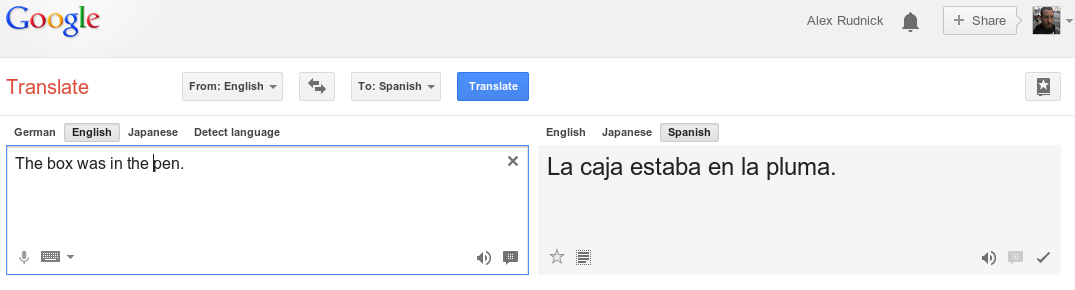
\includegraphics[width=12cm]{box-in-pen.png}
  \caption{Google Translate, September 17, 2013; interestingly, adding or
  removing the final period in the English sentence causes a switch between the
  ``pluma" and ``corral" renderings.}
  \label{fig:box-in-pen}
\end{figure}


\begin{quote}
During the past year I have repeatedly tried to point out the illusory
character of the FAHQT ideal even in respect to the mechanical determination of
the syntactical structure of a given source-language sentence... Here I shall
show that there exist extremely simple sentences in English -- and the same
holds, I am sure, for any other natural language -- which within certain
linguistic contexts, would be uniquely (up to plain synonymy) and unambiguously
translated into any other language by anyone with a sufficient knowledge of the
two languages involved, though I know of no program that would enable a machine
to come up with this unique rendering unless by a completely arbitrary and
\emph{ad hoc} procedure whose futility would show itself in the next example.

A sentence of this kind is the following: \emph{The box was in the pen.}
\end{quote}



\section{Cross-lingual word sense disambiguation}
\label{sec:clwsd}

Cross-lingual word sense disambiguation (CL-WSD) is the task of labeling words
or phrases in some input text with their contextually-appropriate translations
into some target language.
It is a variant of the more general WSD task, with the sense inventory for each
word defined as its possible translations.
This setting for WSD has immediate applications in both machine translation and
cross-language information retrieval, since many words have multiple possible
translations.

WSD in translation has a long history; practical work in integrating
WSD with statistical machine translation dates back to early SMT work at IBM
\cite{Brown91word-sensedisambiguation}, but the problem itself was described in
Warren Weaver's prescient 1949 memorandum \cite{weavermemo}, which describes an
essentially modern conception of word sense disambiguation.


Framing the resolution of lexical ambiguities in machine translation
as an explicit classification
task has a long history, dating back at least to early SMT work at IBM
\cite{Brown91word-sensedisambiguation}.  More recently, Carpuat and Wu have
shown how to use word-sense disambiguation techniques to improve modern
phrase-based SMT systems \cite{carpuatpsd}, even though the language model and
phrase tables of these systems can mitigate the problem of lexical ambiguities
somewhat. Treating lexical selection as a word-sense disambiguation problem, in
which the sense inventory for each source-language word is its set of possible
translations, is often called cross-lingual WSD (CL-WSD). This framing has
received enough attention to warrant shared tasks at recent SemEval workshops;
the most recent running of the task is described in \cite{task10}.





In general, there is a many-to-many relationship between words across language
boundaries.
This happens for a number of reasons: figurative or metaphorical uses may not
translate directly,
obligatory information in one language may be left unspecified in another,
or the criteria for selecting a word may simply differ.
To give some familiar examples, a ``leg" of a trip in English is typically
translated as \emph{etape} in French, which is unrelated to limbs used for
walking;
translating ``brother" to Japanese requires specifying whether the brother is
older (\emph{ani}) or younger (\emph{ot\=oto});
a soap bubble or a ceramic plate can be destroyed with the same word in
Chinese, whereas English speakers typically distinguish between the verbs
``pop" and ``break" \cite{majid2007semantic}.

Despite these difficulties, most statistical MT systems do not use an explicit
WSD module \cite{wsdchap3}; the language model and phrase tables of these
systems mitigate lexical ambiguities by encouraging words used collocationally
to appear together in the output. Entire phrases\footnote{Not necessarily
``phrases" in a syntactic sense, but subsequences of sentences} such as verbs
with their common objects may be learned and stored in the phrase table, and
the language model will encourage common collocations as well.

To take a look at some apparently easier examples, let us also consider the
following usages of \emph{letter}, from the test set of a recent SemEval shared
task \cite{task10}, and how to translate them into Spanish.

\enumsentence{
But a quick look at today's \emph{letters} to the editor in the Times suggest
that here at least is one department of the paper that could use a little more
fact-checking. }
\label{sent:carta}
\enumsentence{
All over the ice were little Cohens, little Levys, their names sewed in block
\emph{letters} on the backs of their jerseys. }
\label{sent:letra}

We would want (\ref{sent:carta}) to be translated with the word \emph{carta},
and (\ref{sent:letra}) to be translated with \emph{letra} or something similar.
Google Translate (as of this writing) handles both of these sentences well,
rendering the first with ``cartas" and the second with an even better choice,
translating the phrase ``block letters" as \emph{mayúsculas}.
However longer-distance relationships, search errors, or simple statistical
accidents can still cause strange translations in practice.

Despite the great success of SMT systems without any explicit models for WSD,
there has been recent interest in CL-WSD and its application to translation
systems, sparking shared tasks at recent SemEval workshops
\cite{lefever-hoste:2010:SemEval,task10} and a number of other projects
described in some detail in \S\ref{sec:relatedwork}).

In this dissertation, we will describe in detail some new approaches for CL-WSD
and how to integrate them into a practical machine translation system.
We will develop and extend at least two broad approaches for CL-WSD: the use of
multilingual evidence where available, and CL-WSD as a sequence labeling
problem.
Both of these techniques have been prototyped and presented at workshops, but
they will be refined significantly and packaged into more general tools for use
in MT.  

\begin{figure}
  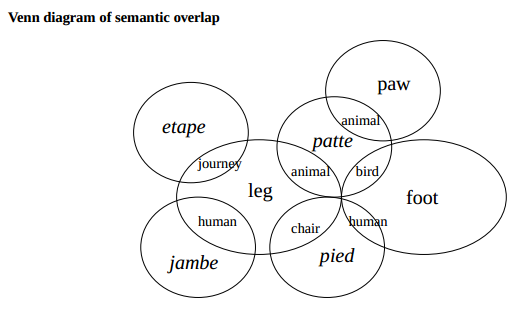
\includegraphics[width=12cm]{hutchins-leg-etc.png}
  \caption{Overlap of words related to ``leg"; relationships between English
  and French words. Figure 21.2 from \protect\cite{slp1}; example originally
  from \protect\cite[Chapter 6]{hutchins1992introduction}.}
  \label{fig:leg}
\end{figure}


\section{History of CL-WSD}
Before the work of Carpuat and Wu~\cite{improvingsmtwsd}, it was apparently
unclear whether WSD was necessary or helpful for a state-of-the-art statistical
MT system; lexical choice among possible translations for a given word can
often be handled by the language model for the target language, simply due to
collocations of appropriate words in the training data.




To our knowledge, there has not been other work on framing CL-WSD for all words
in an input sentence as a sequence labeling problem. However, in monolingual
WSD, Molina \textit{et al.} \cite{DBLP:conf/iberamia/MolinaPS02} have made
use of HMMs for WSD. 


%% Brown et al
Framing the resolution of lexical ambiguities in machine translation
as an explicit classification
task has a long history, dating back at least to early SMT work at IBM
\cite{Brown91word-sensedisambiguation}.

An early paper by IBM researchers \cite{Brown91word-sensedisambiguation},
outlines the CLWSD task in a strikingly similar way, as a WSD task where the
possible senses of a word are extracted from statistical alignments learned
over a bitext corpus. Brown \textit{et al.} report significant translation
quality improvements through the use of their WSD system, over a small
hand-evaluated set of test sentences.







\section{Hybrid MT}

In recent years, we have seen renewed interest in machine translation systems
that take into account syntactic structure, linguistic knowledge, and semantic
representations.
Hopefully, these will provide better translation for language pairs with
significant reordering or syntactic divergences, and where one or both of the
languages has rich morphology.
The boundaries between rule-based and statistical MT systems are becoming
increasingly blurred, and hybrid systems are being developed in both
directions, with RBMT systems incorporating components based on machine
learning, as well as SMT systems making use of linguistic knowledge for
morphology and syntax.

Additionally, for most of the world's language pairs, there is simply no large
bitext corpus available, so training a purely statistical machine translation
system is infeasible.
Thus, while SMT approaches have had great success, and drastically changed the
machine translation landscape since the 1990s, RBMT approaches are still
relevant for many language pairs.

We would like for RBMT or hybrid systems, once developed, to be able to make
use of any bitext on hand.  Like SMT systems, they should be able to produce
better translations as larger corpora become available, without additional code
changes.
In this dissertation work, we will develop a software package called
chipa, which will do just that: %% XXX: better wording?
it will integrate with a variety of machine translation systems to help them
use any available bitext to make better word choices.


%%%% Paraguay and Guarani %%%%
\urldef{\leydelenguas}\url{http://www.cultura.gov.py/lang/es-es/2011/05/ley-de-lenguas-n%C2%BA-4251/}

\section{Paraguay and the Guarani Language}
Guarani is an indigenous language spoken in Paraguay and the surrounding
region.
Historically, it was the native language of the indigenous Guarani people. The
word for the Guarani language in Guarani is \emph{avañe'e} (``people's
language", where \emph{ñe'e} means ``language").

Guarani is unique among indigenous American languages in that a substantial
number of non-indigenous people speak it.  The majority of Paraguayans are
conversant in Guarani, although they are likely to be bilingual with Spanish.
In practice, many Paraguayans use a combination of Guarani and Spanish called
\emph{Jopar{\'a}}, which is the Guarani word for ``mixture".

Paraguay is officially a bilingual, pluricultural country, as described by its
famous \emph{Ley de Lenguas} \footnote{\leydelenguas} (``Law of Languages").
However, the Guarani language is at a significant social and economic
disadvantage and is typically not used in formal situations, as Spanish is
often considered more prestigious. There are, however, an engaged activist
community, many Guarani-language educators, and a government agency devoted
specifically to policy regarding language.
The Guarani language figures significantly into a sense of Paraguayan national
identity and history.

Guarani has a rich, polysynthetic, agglutinative morphology, in which roots can
derive into different parts of speech, and often several roots can combine into
a single word. Guarani morphology can mark tense, aspect (even on nouns),
number, negation, and other features. However, unlike Spanish, it has no
grammatical gender.  Guarani's rich morphology can make many NLP tasks,
including ones seemingly as simple as spell-checking, rather challenging.

We are in contact with a number of collaborators in Paraguay, including
language activists and educators from the \emph{Ateneo de la Lengua y Cultura
Guaraní} \footnote{\url{http://www.ateneoguarani.edu.py/}} and the
\emph{Fundación Yvy Marãe'{\~y}} \footnote{\url{http://yvymaraey.org/}},
both of which are schools that offer training for Guarani-language translators.

We have also started discussing development plans with several local software
developers -- including some from the local One Laptop Per Child organization
-- interested in building open source software, such as the corpus-building
websites described in the next section.



\subsection{Online Language Tools for Guarani}
There are currently very few online language tools for Guarani; some of the
best available ones are iGuarani \footnote{\url{http://iguarani.com/}}, a
searchable online dictionary and gisting translation system developed by young
Paraguayan programmer Diego Alejandro Gavilán.

There is also a small searchable online dictionary developed by Wolf Lustig
\footnote{\url{http://www.uni-mainz.de/cgi-bin/guarani2/dictionary.pl}},
which has versions in Spanish, German, and English. He has graciously made this
dictionary available for our use, and this will provide a starting point for
our Spanish-Guarani translation system.

The Guarani activist and education community has a presence on the Web,
although a startlingly large fraction of this presence is a single author,
Dr. David Galeano Olivera, the president of the \emph{Ateneo de Lengua y
Cultura Guaraní}. He has collected a number of resources both about and in the
Guarani language
\footnote{\url{http://cafehistoria.ning.com/profiles/blogs/la-lengua-guarani-o-avanee-en}},
some in Spanish and some in Guarani, and will likely continue to do so.
